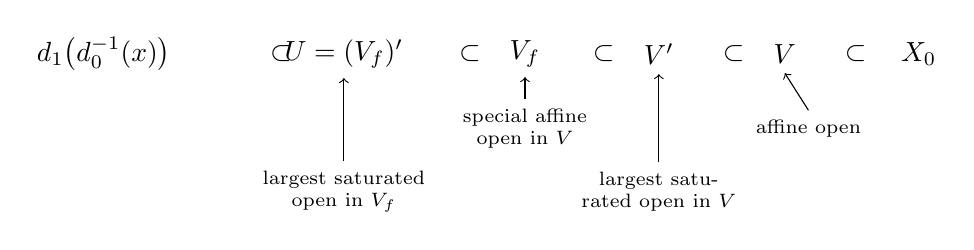
\begin{tikzpicture}[
  baseline=(current bounding box.center),
  every node/.style={font=\normalsize},
  annotation/.style={align=center,font=\scriptsize,text width=2.4cm}
]
\node (fiber) at (0,0) {\(d_1\!\left(d_0^{-1}(x)\right)\)};
\node at (2.25,0) {\(\subset\)};
\node (u) at (3.05,0) {\(U=(V_f)'\)};
\node at (4.65,0) {\(\subset\)};
\node (vf) at (5.35,0) {\(V_f\)};
\node at (6.35,0) {\(\subset\)};
\node (vp) at (7.05,0) {\(V'\)};
\node at (8.00,0) {\(\subset\)};
\node (v) at (8.65,0) {\(V\)};
\node at (9.55,0) {\(\subset\)};
\node at (10.35,0) {\(X_0\)};
\node[annotation] (largestvf) at (3.05,-1.75)
  {largest saturated open in \(V_f\)};
\node[annotation] (specialv) at (5.35,-0.95)
  {special affine open in \(V\)};
\node[annotation] (largestv) at (7.05,-1.75)
  {largest saturated open in \(V\)};
\node[annotation] (affinev) at (8.95,-0.95)
  {affine open};
\draw[->] (largestvf.north) -- (u.south);
\draw[->] (specialv.north) -- (vf.south);
\draw[->] (largestv.north) -- (vp.south);
\draw[->] (affinev.north) -- (v.south);
\end{tikzpicture}
